\newpage
\section{Project description}

\subsection{Research background}

\subsubsection{Blockchain and scalability problem}
While the demand for blockchain solutions is increasing over years since the
first introduction of Bitcoin, the performance of mainstream blockchains is
still a barrier to the adoption of blockchain technology. As a global payment
system, Visa is capable of processing around 24,000 transactions per second on
average \cite{visa}, while the number is 7 and 15 for Bitcoin and Etherum
respectively \cite{ethereum:sharding, nakamoto2019bitcoin}. Scaling the
performance of blockchain systems has become a hot topic for both industry and
academia, with many proposals. Those proposals varies from optimizing the
performance of the consensus protocols \cite{dang2019towards}, partitioning the
blockchain \cite{wang2019sok} to shifting the computation from the blockchain
(on-chain) to the outside (off-chain) \cite{teutsch2019scalable,
network2018cheap}. Being the first generation of blockchain, Bitcoin has very
limited support for programmable transactions, thus also has limited options for
scaling that doesn't require changes in its protocol. On the other hand, later
generations of blockchain (Etherum, NEO, Stellar, etc.) address this problem by
providing a general purpose programmable infrastructure (as known as smart
contract), where the blockchain does not only store financial data but also have
the capability of deploying and executing custom code on the blockchain system.
This increases the flexibility of the system and enable more options for
optimization.

\subsubsection{Scaling by partitioning}
Among all proposed method for scaling the performance, sharding the blockchain
state is an effective and practical solution, as it can overcome both
performance and scalability problems of blockchain. Partitioning (or
\emph{sharding}) is a technique that divides the state of a service or a system
in multiple partitions so that most requests or transactions access one
partition only and are equally distributed among partitions. As a result,
partitions can work in parallel to maximize the performance and improve the
throughput. On the downside of this approach, if a transaction accesses data
from multiple partitions, those partitions have to coordinate to execute the
transaction, thus increase the cost of the execution. The major challenge in
this approach is to come up with an optimized partitioning scheme to minimize
the number of cross-partition transactions, and also an effective execution
scheme that could handle multi-partition transactions.

\subsubsection{State machine replication (SMR) and Scaling SMR}
State machine replication, also called active replication, is a common approach
to building fault-tolerant systems \cite{Lam78, Sch90}. Participants in a
replicated state machine system form agreement on a sequence of transactions and
apply them in sequence order deterministically to the reach the same state. With
its simple yet effective execution model, state machine replication is at the
core of many blockchain systems \cite{baudet2019state, cachin2016architecture}.
In terms of scalability, unfortunately, classic state machine replication does
not scale. Increasing the number of replicas will not scale performance since
each replica must execute every command. In the work called Dynamic scalable
state machine replication (\dssmr), Le \emph{et al.} proposed an approach for
scaling the performance of SMR by allowing SMR system to reconfigure its data
placement on-the-fly. By moving data ``on demand'' to maximize the number of
single partition requests, \dssmr{} allows SMR system to adapt the partitioning
scheme as workloads change. To keep track the partition of objects in the
system, \dssmr{} maintain a location oracle with a global view of the
application state. The result of this work shows that scalable performance could
be achieved in a replication system with a good partitioning scheme. In a later
work, the authors introduced \dynastar, an optimized partitioning solutions for
SMR. \dynastar shows that by using the data of the location oracle to come up
with an optimized partitioning, scalable performance is achievable for
real-world application. The authors also presented a detailed experimental
evaluation of \dynastar using the TPC-C benchmark and a social network service
populated with a real social network graph. Figure \ref{fig:tpcc} shows the
performance evaluation of \dynastar with TPC-C benchmark. Figure
\ref{fig:tpcc}(a) depicts the impact of partitioning on the performance of a
system before and after an optimized partitioning configuration is applied.
Figure \ref{fig:tpcc}(b) shows the scalability of \dynastar when increase the
size of the system (adding more data and computational resources). It's worth to
note that in a TPC-C benchmark, the average rate of mutli-partition transactions
is 15\%.

\begin{figure*}[ht!]
  \centering
  \begin{subfigure}{.48\textwidth}
    \centering
    \includegraphics[width=0.8\columnwidth]{figures/tpcc-detail-dynastar}
  \caption{Repartitioning in \dynastar; throughput (top), objects exchanged
  between partitions (middle), and percentage of multi-partition commands
  (bottom).}
  \end{subfigure}
  \begin{subfigure}{.48\textwidth}
    \centering
    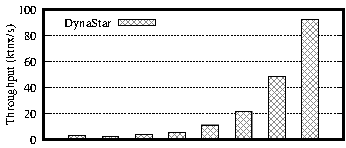
\includegraphics[width=\textwidth]{./figures/tpcc-scaling-tp-lat-bridge}
    \caption{Performance scalability with TPC-C. Throughput (in thousands of transactions per second, ktps)}
  \end{subfigure}
  \caption{Dynastar performance with TPC-C Benchmark}
  \label{fig:tpcc}
\end{figure*}

\subsection{Innovation potential and market review} 

\subsubsection{General ideas}

\subsubsection{General ideas}

\subsubsection{Integrability}
This proposal is based on an assumption that contracts and data can move across
blockchain. Moving and sharing data across blockchain systems or between
partitions in a blockchain (interoperability) has been in the blockchain
wishlist for some time. A protocol with this goals has been proposed in the
Ethereum research forum concurrently with the development of this work
\cite{buterin2018yanking}. In another work, a move primitive introduced by Fynn \emph{et al.}
\cite{fynn2020move} allows programmable blockchains to interoperate by moving
contracts and data from one to another. This solution is plugable as a smart
contract, requires no modification to the blockchain. 

With the on-chain component in the form of smart contract, our proposed system
could be integrated to existing blockchain systems easily without any change in
the blockchain protocol. 

\subsubsection{Expected outcome}

In an analysis in \cite{fynn2020move}, the author performed an extensive study
on the impact of partitioning Ethereum blockchain. The study showed that even on
a workload that was not created for a sharded system, the partitioning scheme
could achieve a rate of less then 10 percents of cross partition transaction. 


\subsection{Implementation strategy}

\subsection{Project plan}

